%!TEX root = ../Demo.tex
\chapter{介绍}
随着虚拟化技术的吸引力越来越大,云计算的发展,数据中心越来越受到业界和学术界的关注。云提供商使用数据中心虚拟化技术将物理数据中心资源划分为虚拟数据中心(VDC),以共享物理资源。每个VDC都可以为用户提供相关服务。通常,VDC是虚拟资源(例如,虚拟机(VM),虚拟交换机,虚拟路由器或虚拟链路)的集合。同时,VDC请求通常与服务提供商签订服务水平协议(SLA)。因此,在将VDC请求映射到物理数据中心时,必须满足SLA(例如,传输延迟,资源需求等)。

但是,由于用户需求的增加,单个数据中心可能无法为不断增加的用户请求提供资源。因此,已经提出了联合多个数据中心以提供VDC请求的概念,并且云服务提供商因此在多个数据中心中向用户供应虚拟化资源\cite{jin2012efficient,amokrane2013greenhead,xu2015rethink}。此外,随着数据中心的功耗和物理资源(例如,CPU,存储,存储器或带宽)消耗的增加,节省能源和提高资源利用率已逐渐成为工业界或学术界的热门话题。此外,为了避免因缺乏网络资源而导致的SLA违规,研究人员在单个数据中心或多个数据中心提出了各种VM迁移方法\cite{adami2013virtual,aiash2014secure,zhang2013scheduling,cerroni2014multiple,callegati2013live,sarker2013performance}。这些VM迁移方法允许研究人员使用适当的迁移策略来实现节约能源,提高资源利用率和避免违反SLA的目的。

为了减少虚拟机的迁移时间并加快迁移过程,\cite{zhang2013scheduling}中的作者研究并建模了多个虚拟机迁移问题,并提出了一种有效的云计算虚拟机迁移调度方法。虽然调度方法可以迁移多个虚拟机,但作者没有考虑虚拟机之间的相关性。

但是,实际上,为了节省能源和维护系统,云提供商通常需要迁移多个相关的虚拟机或迁移整个VDC请求。例如,在\cite{cerroni2014multiple,callegati2013live}中,Walter Cerroni等人。研究了迁移一组协作虚拟机的问题,并提出了迁移多个虚拟机的串行和并行迁移策略。作者比较了迁移多个VM的串行和并行迁移策略的迁移时间和停机时间。但是,他们没有研究VM迁移的资源分配或配置问题。在\cite{sarker2013performance}中,作者还清楚地说明了多个虚拟机之间的关联,并提出了一种算法来重新映射虚拟机,计算迁移路径和调度多个数据中心的迁移带宽,然而,该算法的主要目标是计算迁移路径和调度迁移带宽而不是重新映射VM。

因此,要优化多个相关虚拟机或VDC迁移的迁移性能请求,有必要设计一个新的迁移算法。在本文中,我们研究了在多个数据中心中迁移多个相关虚拟机的问题。由于多个相关虚拟机属于同一VDC请求,因此我们将整个VDC请求或VDC请求的一部分虚拟机视为迁移请求。我们提出了一种实时在线迁移算法VDC-M,用于在多个数据中心之间迁移VDC迁移请求。最后,我们使用美国国家科学基金会(NSF)网络作为基板网络进行广泛的模拟,以评估我们提出的算法的性能。仿真结果表明,该算法在总VDC重映射成本,阻塞率,平均迁移时间和平均停机时间方面具有良好的应用前景。

在本文的其余部分安排如下。在第2节中,我们讨论了相关的工作。在第3节中,我们提出了在这项工作中研究的问题的表述。我们在第4节中提出了启发式方法,继续对第5节中获得的模拟结果进行评估和分析。我们在第6节中总结了本文。

\chapter{相关工作}

\section{单个VM迁移}
为了降低违反SLA的可能性,云提供商可能需要通过迁移虚拟机来保证服务质量(QoS)。此外,云提供商还可以通过迁移和整合虚拟机来节省能源并提高资源利用率。

对离线或在线单虚拟机迁移问题进行了一些研究\cite{khazaei2013performance,zhang2014delay,ding2015energy,rao2015heuristics,chen2014consolidating,mohamed2015autonomic,xu2013enhancing,huang2013multi}。自生存性要求以来,研究人员已将研究方向转向实时迁移。因此,一些关于虚拟机迁移的现有研究提出了最小化迁移时间和停机时间的策略。例如,[10],[11],[12]中的作者提出并实施了在线或实时迁移策略来迁移虚拟机,以最大限度地减少虚拟机停机时间。在[13]中,作者提出了单个虚拟机迁移过程的性能分析模型,以分析虚拟机的迁移时间和停机时间。在\cite{zhang2014delay}中,作者研究了应该提供多少带宽以保证实时VM迁移的总迁移时间和停机时间的问题。

除了优化和测量迁移时间和停机时间外,研究人员还提出了一些相关的虚拟机迁移算法来实现其他目标。例如,在\cite{ding2015energy}中,作者提出了一种能量有效的虚拟机调度算法,以减少云消耗的总能量,同时也很好地支持动态电压和频率调整。在\cite{rao2015heuristics}中,为了降低总体成本和能耗,作者提出了以低能耗和SLA违规进行碎片整理的方法。在\cite{chen2014consolidating}中,为了在保证服务水平协议的同时最大化能源效率和云资源利用率,作者提出了虚拟机迁移和合并算法。在\cite{mohamed2015autonomic}中,为了保证QoS和减少支出,作者提出了一种自动管理模型来有效地安排云资源,并降低了费用。在\cite{xu2013enhancing}中,为了提高虚拟机的生存性,作者提出了一种虚拟机备份和迁移算法;当原始VM发生故障时,应用程序/任务将迁移到备份VM并继续运行。在\cite{huang2013multi}中,作者提出了一种虚拟机迁移算法,以减少迁移引起的网络负载。这些关于虚拟机迁移的研究通常针对单个虚拟机迁移问题,而大多数针对单个数据中心。因此,这些研究不适用于多个数据中心之间多个VM迁移的场景。

\section{多个虚拟机迁移}
随着虚拟机迁移技术的发展,近年来,一些研究人员试图解决多虚拟机迁移问题。

在\cite{zhang2013scheduling}中,作者分析并建模了多个虚拟机迁移问题,并提出了一种调度方法,以减少虚拟机的迁移时间,从而加速迁移过程。在\cite{keller2012live}中,作者将应用程序从一个位置迁移到另一个位置。由于应用程序通常是一组多个相关的虚拟机,因此作者将应用程序作为一个整体进行迁移,然后测量出迁移时间和停机时间。在\cite{atif2014adaptive}中,作者使用Xen 3.3.0进行了模拟实验,并在作业从一个子集迁移到另一个子集时测试了迁移时间和其他相关参数。在\cite{yang2014method}中,作者提出了一种管理虚拟机集群迁移的方法。当用于托管虚拟机的源物理机的可用资源量接近阈值时,虚拟机群集将迁移到新的物理机。在\cite{xu2013iaware}中,为了避免违反SLA的可能性,作者提出了iAware方法,一种轻量级的干扰虚拟机实时迁移策略。

尽管\cite{zhang2013scheduling,keller2012live,atif2014adaptive,yang2014method,xu2013iaware}中提出的算法适用于多个虚拟机迁移或虚拟机群集迁移问题,但作者没有考虑虚拟机之间的相关性。实际上,云提供商通常需要迁移多个相关的虚拟机或迁移整个VDC请求以实现优化目标。例如,在\cite{cerroni2014multiple,callegati2013live}中,作者研究了迁移协作虚拟机组的问题。

然而,虽然\cite{cerroni2014multiple,callegati2013live}中的作者提出了多个相关虚拟机的串行和并行迁移策略,但他们没有研究迁移过程中多个虚拟机的资源分配或配置问题。该研究[9]解决了在多个数据中心迁移多个相关虚拟机的问题,尽管作者提出了重新映射虚拟机,查找迁移路径和在多个数据中心中调度迁移带宽的算法,该算法的主要目标是查找迁移路径和计划迁移带宽而不是重新映射虚拟机。因此,很少有VDC或多个相关的VM迁移算法,尤其适用于研究重新映射VDC迁移请求。
因此,本文中提出VDC-M算法以解决在多个数据中心之间在线迁移VDC或多个相关虚拟机的问题至关重要。

\chapter{问题陈述和公式}

\section{问题陈述}
我们研究了在多个数据中心中迁移多个相关虚拟机的问题。我们考虑需要将多个相关虚拟机从源服务器迁移到新目标服务器的情况。多个相关的虚拟机是一组虚拟机,而所有虚拟机都通过虚拟链接连接。由于多个相关的虚拟机属于VDC请求,因此这些多个相关的虚拟机要么是整个VDC请求,要么是VDC请求的一部分虚拟机。因此,在这项工作中,可以将多个相关的虚拟机表示为VDC迁移请求。

具体来说,鉴于由多个数据中心组成的物理数据中心(在本文中可互换地称为基板网络)具有由核心网络互连的不同位置,需要迁移VDC迁移请求,并且原始映射为VDC请求,问题是如何有效地将包括在VDC请求中的这些相关虚拟机迁移到目标物理服务器,使得重新映射的成本,阻塞率,总迁移时间和总停机时间最小化,同时满足所有迁移约束。

\section{VDC迁移请求}
我们将VDC迁移请求建模为无向加权图。迁移请求的示例如图1所示。在此示例中,虚拟机旁边的矩形中的数字表示服务器资源要求,虚拟机内存大小和迁移带宽要求以及旁边的数字。虚链路表示链路资源需求和可容忍的传输延迟。

\section{VDC迁移}
VDC迁移可分为两个阶段。第一阶段是为VDC迁移请求重新分配资源,即重新映射VDC迁移请求。第二阶段是查找迁移路径并为这些迁移路径分配带宽资源,然后将每个虚拟机从源服务器迁移到目标服务器。在VDC迁移请求的重新映射过程中,我们需要为VDC迁移请求的每个虚拟机分配不同的基板服务器和所需的计算资源,并映射VDC迁移请求的每个虚拟链路。上述VDC重新映射过程可以如下公式化。

\subsection{虚拟机重映射}
虚拟机重映射的过程可表示为:

\begin{figure}[!htb]
  \centering
  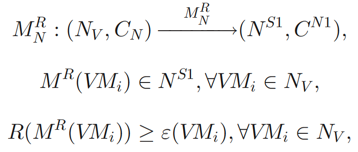
\includegraphics{./Figure/express1.png}
\end{figure}

\subsection{VDC链路重映射}
VDC链路的映射可以表示为:

\begin{figure}[!htb]
  \centering
  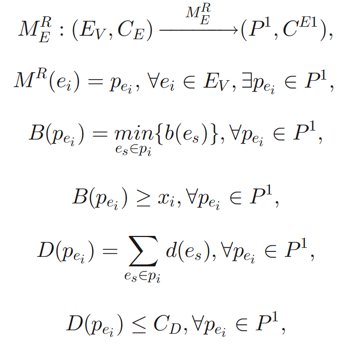
\includegraphics{./Figure/express2.png}
\end{figure}

在迁移过程中,我们必须计算迁移路径并分配迁移带宽,以将虚拟机从源服务器迁移到目标服务器。该过程可表示为:

\begin{figure}[!htb]
  \centering
  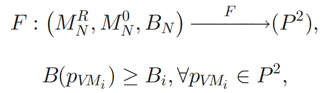
\includegraphics{./Figure/express3.png}
\end{figure}

\begin{figure}[!htb]
  \centering
  \includegraphics[{./Figure/Fig3.png}
  \caption{一个VDC迁移实例}\label{Fig1}
\end{figure}

图\ref{Fig1}显示了重新映射和迁移VDC迁移请求的示例。在此示例中,VDC迁移请求最初映射到数据中心A和C,如图中黑色虚线框所示。在重映射过程中,VDC迁移请求被映射到数据中心B和D,如图\ref{Fig1}中的红色实心框所示.

\section{VDC迁移时间}
我们使用预复制策略迁移单个虚拟机。对于多个虚拟机,我们使用并行迁移策略。单个虚拟机的迁移时间和停机时间与\cite{callegati2013live}类似。

\begin{figure}[!htb]
  \centering
  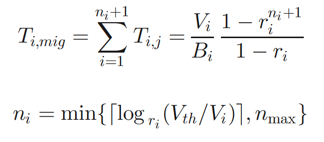
\includegraphics{./Figure/express1_2.png}
\end{figure}

在本文中,我们关注迁移由多个相关虚拟机组成的VDC迁移请求的问题。为了提高效率,我们采用并行迁移策略来迁移多个VM。在迁移过程中,每个虚拟机都有自己独立的迁移带宽。因此,整个VDC迁移请求的迁移时间是上次完全迁移的虚拟机的迁移时间。

\begin{figure}[!htb]
  \centering
  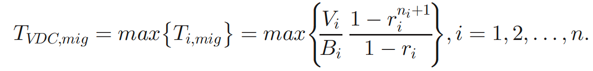
\includegraphics{./Figure/express6.png}
\end{figure}

\chapter{启发式算法}
我们提出了VDC迁移(VDC-M)算法,用于解决请求动态到达的多个VDC请求的在线迁移问题。我们提出的算法首先重新映射VDC迁移请求,然后查找迁移路径并分配带宽资源,以将虚拟机从源服务器迁移到目标服务器。在不失一般性的情况下,我们假设VDC请求在此工作中根据泊松过程到达。在VDC-M算法中,所有到达VDC迁移请求首先在队列中缓冲,表示为ArrivedVDC。我们将ExpiredVDC定义为过期的VDC迁移请求集。 

ArrivedVDC队列中的每个VDC迁移请求都将被重新映射并逐个迁移。队列ArrivedVDC中的某些请求可能由于缺少资源而被阻止。我们将VDCblo定义为阻止迁移请求的集合。
VDC-M算法的主要步骤包括重新映射VDC,计算迁移路径和为迁移路径分配带宽。在VDC-M算法中,当VDC迁移请求到达时,它首先调用VDC重新映射(RM)过程以重新映射VDC迁移请求,然后调用VDC路由和带宽分配(RBA)过程来计算迁移路径,以及最后为迁移路径分配带宽资源并迁移VDC。算法1中显示了所提出的迁移算法的伪代码。

\begin{figure}[!htb]
  \centering
  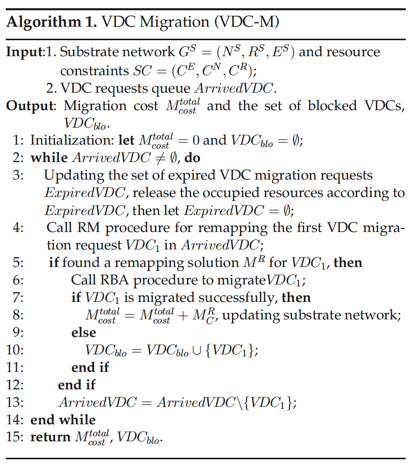
\includegraphics{./Figure/Other1.png}
\end{figure}

路由和带宽分配过程用于计算迁移路径并为它们分配带宽资源。它根据原始映射记录和每个虚拟机的重映射记录以及带宽要求找到迁移路径并分配迁移带宽,然后计算迁移时间和VDC迁移请求的停机时间。详细的RBA程序显示在程序2中。

\begin{figure}[!htb]
  \centering
  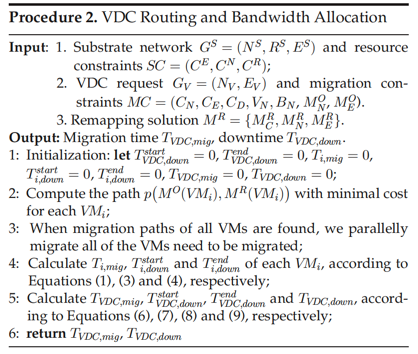
\includegraphics{./Figure/Other2.png}
\end{figure}

\chapter{仿真结果}
我们通过大量的仿真来评估所提算法的性能。在本节中,我们首先介绍仿真环境,然后描述在我们的仿真中使用的几个性能参数。最后,我们描述了我们的主要模拟结果和分析。

\section{仿真环境}
在我们的仿真中,我们使用美国的NSF网络作为基板网络,有7个数据中心连接到美国的NSF网络,如图\ref{Fig2}所示。

\begin{figure}[!htb]
  \centering
  \includegraphics[{./Figure/Fig4.png}
  \caption{美国的NSF网络}\label{Fig2}
\end{figure}

数据中心有一个树拓扑\cite{fang2013power},如图\ref{Fig3}所示。

\begin{figure}[!htb]
  \centering
  \includegraphics[{./Figure/Fig5.png}
  \caption{树拓扑}\label{Fig3}
\end{figure}

在本文中,为了扩展我们算法的范围,我们使用随机生成的VDC迁移请求而不是两层树拓扑。

在资源容量有限的情况下,基板服务器的计算资源容量遵循从8到10个单元的均匀分布。我们参考参考文献\cite{alizadeh2013pfabric}。 设置数据中心内物理链路的带宽容量。在每个数据中心,直接连接服务器的物理链路的带宽容量为10 Gbps,路由器到路由器物理链路的带宽容量为40 Gbps。每个核心网链路的带宽容量为100 Gbps。在不失一般性的情况下,我们假设:i)每单位服务器资源成本和单位链路带宽成本均为1个单位; ii)每个核心网链路的传输延迟为1个单元; iii)内部数据中心中的每个链路都没有传输延迟。

此外,在我们的模拟中,我们假设VDC迁移请求在泊松过程之后到达,每个VDC迁移请求中的虚拟机数量在6,12,24和36之间变化;每个VDC迁移请求的服务器资源需求遵循均匀分布U(1.3,1.5),U(0.6,0.8),U(0.2,0.4)或U(0.1,0.3);每个VDC迁移请求的链路资源要求也遵循均匀分布U(1.3,1.5),U(0.6,0.8),U(0.2,0.4)或U(0.1,0.3)。每个虚拟机的迁移带宽为1 Gbps,每个链路的传输延迟约束为四个时间单位。

关于VM迁移问题的大多数研究仅考虑单个VM迁移,尽管存在多个VM迁移算法,但它们不考虑这些虚拟机之间的相关性。因此,这些现有算法与我们在这项工作中提出的方法不具有可比性。 \cite{xu2013iaware}中的作者研究了多个虚拟机迁移的问题,然而,\cite{xu2013iaware}的目标与我们的不同。为了实现公平比较,我们扩展和修改\cite{xu2013iaware}中提出的算法如下:i)我们用我们的方法取代\cite{xu2013iaware}的目标; ii)我们将虚拟链路重新映射过程添加到\cite{xu2013iaware}中提出的算法中。扩展算法在我们的仿真结果中表示为VDC-SM。

\section{性能指标}
我们使用以下指标来评估我们在模拟中提出的算法的性能。在无限资源容量的情况下,我们测量总重映射和迁移成本,总迁移成本,总重映射成本,核心网络中的VDC重映射成本,数据中心的VDC重映射成本,平均迁移时间和平均停机时间。在资源容量有限的情况下,我们还测量阻塞率。

\begin{enumerate}
    \item VDC重新映射和迁移成本总额:使用基础网络资源重新映射和迁移所有VDC迁移请求的总成本。它可以如公式所计算。

    \begin{figure}[!htb]
    \centering
    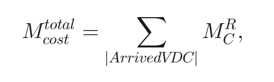
\includegraphics{./Figure/express15.png}
  \end{figure}

    \item 总VDC迁移成本:使用基础网络资源迁移所有VDC迁移请求的总成本。

    \begin{figure}[!htb]
    \centering
    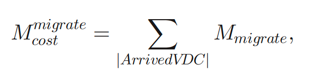
\includegraphics{./Figure/express16.png}
  \end{figure}

    \item 总VDC重映射成本:使用基板网络资源重新映射这些VDC迁移请求的总成本。

    \begin{figure}[!htb]
    \centering
    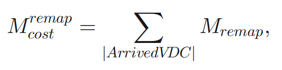
\includegraphics{./Figure/express17.png}
  \end{figure}

    \item 核心网中的VDC重映射成本:使用核心网资源重新映射VDC迁移请求的成本。

    \begin{figure}[!htb]
    \centering
    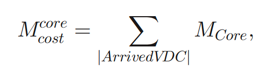
\includegraphics{./Figure/express18.png}
  \end{figure}

    \item 数据中心的VDC重映射成本:使用数据中心内资源重新映射所有VDC迁移请求的成本。

    \begin{figure}[!htb]
    \centering
    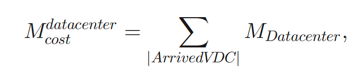
\includegraphics{./Figure/express19.png}
  \end{figure}

    \item 平均迁移时间:每个虚拟机的迁移时间可以用公式以下计算。

    \begin{figure}[!htb]
    \centering
    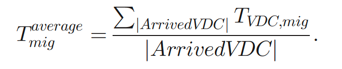
\includegraphics{./Figure/express20.png}
  \end{figure}

    \item 平均停机时间:每个虚拟机的停机时间可以按公式以下计算。

    \begin{figure}[!htb]
    \centering
    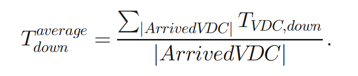
\includegraphics{./Figure/express21.png}
  \end{figure}

\end{enumerate}

\section{仿真结果和分析}
图\ref{Fig4}比较了VDC-M算法和VDC-SM算法的总VDC重映射和迁移成本,其中虚拟机的数量(即n)在6,12,24和36之间变化从图6中可以看出,VDC-M算法的总VDC重映射和迁移成本低于VDC-SM算法。这是因为VDC-M算法可以提供多个候选重映射解决方案,然后以最小成本找到最优解决方案作为最终重映射解决方案。并且VDC-M算法的候选重映射解决方案多于VDC-SM算法的候选重映射解决方案。因此,VDC-M算法比VDC-SM算法更有可能实现更低的重映射和迁移成本。

\begin{figure}[!htb]
    \centering
    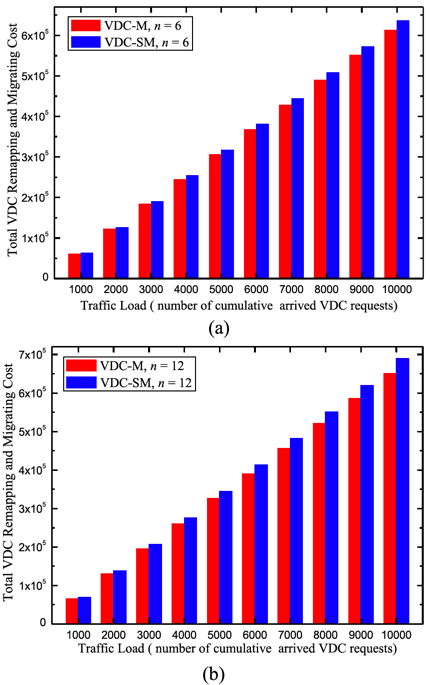
\includegraphics{./Figure/Fig6-1.png}
  \end{figure}
\begin{figure}[!htb]
  \centering
  \includegraphics[{./Figure/Fig6-2.png}
  \caption{VDC-M算法和VDC-SM算法的总VDC重映射和迁移成本}\label{Fig4}
\end{figure}

图\ref{Fig5}描述了当虚拟机的数量在6,12,24和36之间变化时VDC-M算法和VDC-SM算法的总VDC迁移成本。如图\ref{Fig5}所示,我们可以看到VDC-M算法的总VDC迁移成本低于VDC-SM算法。这是因为VDC-M算法在重映射过程中考虑了每个VM的迁移成本,而VDC-SM算法在重映射过程中不考虑这一点。此外,VDC-M算法提供了比VDCSM更多的候选重映射解决方案。因此,VDC-M算法的迁移成本低于VDC-SM算法的迁移成本。

\begin{figure}[!htb]
    \centering
    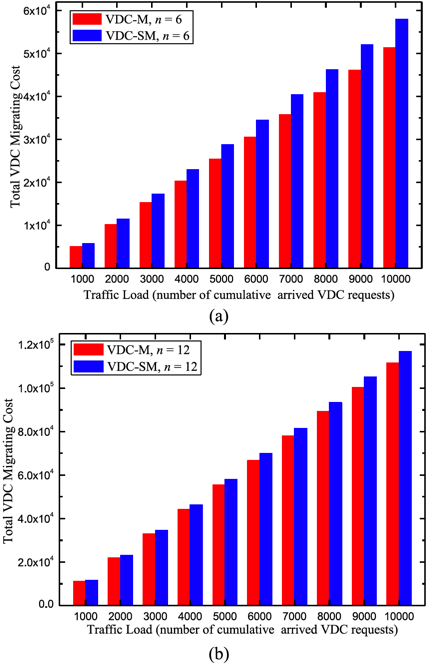
\includegraphics{./Figure/Fig7-1.png}
  \end{figure}
\begin{figure}[!htb]
  \centering
  \includegraphics[{./Figure/Fig7-2.png}
  \caption{VDC-M算法和VDC-SM算法的总VDC迁移成本}\label{Fig5}
\end{figure}

图6比较了VDC-M算法和VDC-SM算法的总VDC重映射成本,其中虚拟机的数量在6,12,24和6之间变化。图6示出了VDC-M算法的总VDC重新映射成本低于VDC-SM算法的总VDC重新映射成本。这是因为VDC-M算法的候选重映射解决方案多于VDCSM算法的候选重映射解决方案。因此,VDC-M算法比VDC-SM算法更有可能实现更低的重映射成本。
从图。从图4,5,6可以看出,VDC-M算法可以同时降低总VDC重映射成本和总VDC迁移成本,从而降低总VDC重映射和迁移成本。

\begin{figure}[!htb]
    \centering
    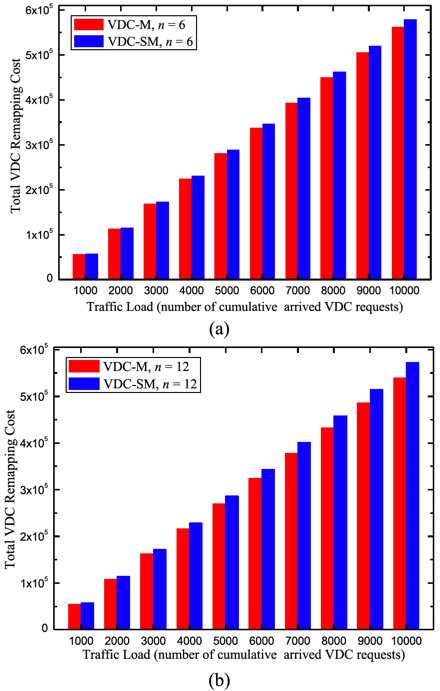
\includegraphics{./Figure/Fig8-1.png}
  \end{figure}
\begin{figure}[!htb]
  \centering
  \includegraphics[{./Figure/Fig8-2.png}
  \caption{VDC-M算法和VDC-SM算法的总VDC重映射成本}\label{Fig6}
\end{figure}

图7显示了VDC-M算法和VDC-SM算法的核心网络中的VDC重映射成本,当虚拟机的数量从12变为36时。当虚拟机的数量为6时,服务器的数量为每个数据中心为16个,所有虚拟机都可以由一个数据中心供应,因此核心网络中的VDC重映射成本为零,并且图7中没有该场景的模拟结果。我们可以看到VDC-M算法的核心网络中的VDC重映射成本低于VDC-SM算法的VDC重映射成本。这是因为在VDC-M算法中,虚拟机将尽可能重新映射到同一数据中心,从而可以减少核心网络中的资源消耗。

\begin{figure}[!htb]
    \centering
    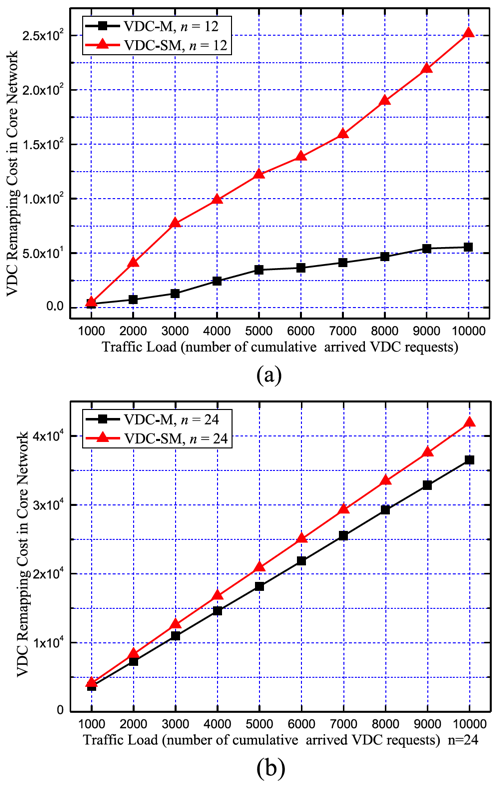
\includegraphics{./Figure/Fig9-1.png}
  \end{figure}
\begin{figure}[!htb]
  \centering
  \includegraphics[{./Figure/Fig9-2.png}
  \caption{VDC-M算法和VDC-SM算法的核心网络中的VDC重映射成本}\label{Fig7}
\end{figure}

图8比较了VDC-M算法数据中心的VDC重映射成本和VDC-SM算法,其中虚拟机数量为12,24或36.当虚拟机数量为6且每个数据中心的服务器数量固定为16时,所有虚拟机可以由一个数据中心容纳,因此VDC重新映射成本为核心网络为零。因此,这两个比较算法的数据中心内的VDC重新映射成本与图8a所示的相同。图8显示当虚拟机的数量从12到36变化时,VDC-M算法的数据中心的VDC重映射成本低于VDC-SM算法的VDC重映射成本。这是因为VDC-M算法可以实现更多候选重映射解决方案比VDC-SM算法更好。因此VDC-M算法不仅有利于降低核心网络中的VDC重映射成本,而且有助于降低数据中心的VDC重映射成本,从而降低总VDC重映射成本。

\begin{figure}[!htb]
    \centering
    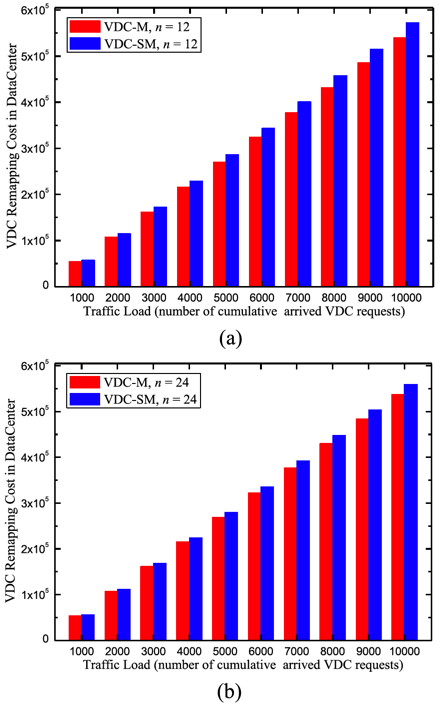
\includegraphics{./Figure/Fig10-1.png}
  \end{figure}
\begin{figure}[!htb]
  \centering
  \includegraphics[{./Figure/Fig10-2.png}
  \caption{VDC-M算法数据中心的VDC重映射成本和VDC-SM算法}\label{Fig8}
\end{figure}

图9显示了VDC-M算法和VDC-SM算法在不同VM内存大小下的平均迁移时间的结果,例如V~U(0.5,1)表示VM内存的大小遵循均匀分布U (0.5,1)。从图9中我们可以看出,在相同的VM内存大小下,VDC-M算法显着减少了平均迁移时间,而不是VDC-SM算法。
由于VDC-M算法以并行方式迁移VM,因此迁移时间是所有虚拟机的最大迁移时间。但是,在VDC-SM中算法,使用串行策略迁移VM,因此迁移时间等于所有虚拟机迁移时间的总和。此外,当虚拟机的数量固定时,两种算法的平均迁移时间随着虚拟机内存大小的增加而增加。这是因为较大的虚拟机内存大小会导致所有虚拟机的内存总量增加,因此需要花费更多时间来完成迁移。

\begin{figure}[!htb]
  \centering
  \includegraphics[{./Figure/Fig11.png}
  \caption{VDC-M算法和VDC-SM算法在不同VM内存大小下的平均迁移时间的结果}\label{Fig9}
\end{figure}

图10显示了比较算法VDC-M和VDC-SM的平均停机时间的模拟结果。
从图中我们可以看出,VDC-M算法的平均停机时间远远低于VDCSM的停机时间,而虚拟机的数量和虚拟机内存的大小算法是一样的。这是因为VDC-M算法使用并行迁移策略在VDC请求中迁移虚拟机,而VDCSM算法采用串行迁移策略。因此,VDC-M算法的平均停机时间远低于VDC-SM算法的停机时间。
此外,当虚拟机内存大小固定时,随着虚拟机数量的增加,VDC-M算法的停机时间会非常缓慢地增加,甚至保持稳定;而VDC-SM算法的平均停机时间增加了随着虚拟机数量的增长。在固定数量的虚拟机中,VDC-M算法的停机时间随着虚拟机内存大小的增加而减小,而VDC-SM算法的停机时间则相反。这是因为这两种算法使用不同的迁移策略,因此导致不同的停机时间。

\begin{figure}[!htb]
  \centering
  \includegraphics[{./Figure/Fig12.png}
  \caption{VDC-M算法和VDC-SM算法在不同VM内存大小下的平均迁移时间的结果}\label{Fig10}
\end{figure}

图11示出了在各种虚拟机号下VDC-M和VDC-SM算法的阻塞比。从图11中可以看出,VDC-M算法的阻塞率远低于VDC-SM算法的阻塞率。这是因为VDC-M算法可以实现比VDC-SM算法更好的重映射解决方案,从而减少资源消耗,并且从长远来看导致更低的阻塞率。

\begin{figure}[!htb]
    \centering
    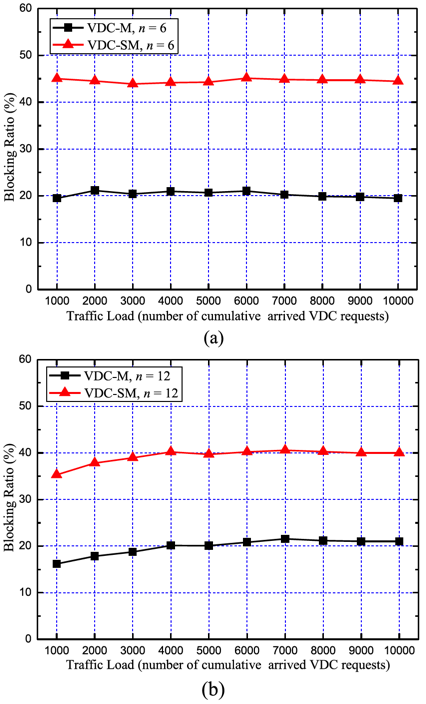
\includegraphics{./Figure/Fig13-1.png}
  \end{figure}
\begin{figure}[!htb]
  \centering
  \includegraphics[{./Figure/Fig13-2.png}
  \caption{各种虚拟机号下VDC-M和VDC-SM算法的阻塞比}\label{Fig11}
\end{figure}

\chapter{结论和讨论}
在本文中,我们研究了多个相关VM的在线实时迁移问题(即VDC迁移请求)。我们设计了一种有效的算法VDC-M来解决这个问题。在VDC-M算法中,我们认为VM之间的相关性包括在VDC迁移请求中,并且整体而不是单独地处理这些相关的VM。在VDC-M算法中,我们首先重新映射VDC迁移请求,然后计算迁移路径并分配带宽资源,以便将虚拟机从源服务器迁移到目标服务器。我们使用美国的NSF网络作为基础网络进行广泛的模拟以评估我们提出的算法的性能。实验结果表明,我们的方法性能优于基准算法VDC-SM,用于在VDC重映射成本,阻塞率,平均迁移时间和平均停机时间方面迁移VDC迁移请求。

然而,为了降低阻塞率和VDC重新映射和迁移成本,VDC-M算法试图提供尽可能多的候选解决方案,从而导致更高的处理时间消耗。因此,我们的方法的时间效率低于VDC-SM算法的时间效率。此外,在我们提出的算法VDC-M中使用并行迁移策略迁移VM,而在VDC-SM算法中使用串行迁移策略逐个迁移VM。因此,对于每个VM的固定带宽迁移路径,在VM迁移期间的特定时间段,我们的算法将导致比VDC-SM算法更重的网络流量负载。





























































































































































































